\section*{Discussion}
We have offered a way around the exploration-exploitation dilemma. We proved the classic dilemma, found when optimizing exploration for reward value, can be resolved by exploring instead for curiosity. In this form the rational trade-off we are left with is solved with a classic strategy taken from game theory: the win-stay lose-shift strategy. When information is more valuable than rewards, then be curious, otherwise seek rewards. We prove this rule has zero formal regret, when maximizing both reward and information value on equal terms.

Arguing the dilemma can be solved without regret is a controversial claim. So we will address some potential criticisms, as a series of questions. The final question explains how this approach can be tested with behavioral experiments. 

\subsection*{Why curiosity?}
Our use of curiosity rests on three well established facts. 1. Curiosity is a primary drive in most, if not all, animal behavior \cite{Inglis2001}. 2. It is as strong, if not sometimes stronger, than the drive for reward \cite{Loewenstein1994,Kidd2015,Gottlieb2018}. 3. Curiosity as an algorithm is highly effective at solving difficult optimization problems \cite{Schmidhuber1991,Pathak2017,Stanton2018,Fister2019,Mouret2015,Colas2020,Cully2015,Pathak2017,Schwartenbeck2019,Laversanne-Finot2018}. 


\subsection*{What about information theory?}
In short, the problems of communication and value are different problems that require different theories.

Weaver \cite{Shannon1964} in his classic introduction to the topic, describes information as a communication problem with three levels. a. The technical problem of transmitting accurately. b. The semantic problem of meaning. c. The effectiveness problem of changing behavior. He then describes how Shannon's work addresses only problem A. It has turned out that Shannon's separation of the problem allowed the information theory to have an incredibly broad application. 

Valuing information is not, at its core, a communications problem. Consider the very simple example Bob and Alice, having a phone conversation and then Tom and Bob having the exact same conversation. The personal history of Bob and Alice will determine what Bob learns in their phone call, and so determines what he values in that phone call. These might be completely different from what he learns when talking to Tom, even if the conversations are identical. What we mean by this example is that the personal history defines what is valuable on a channel, and this is independent of the channel and the messages sent. We have summarized this diagrammatically, in Fig.~\ref{fig:info1}.

\begin{figure}
	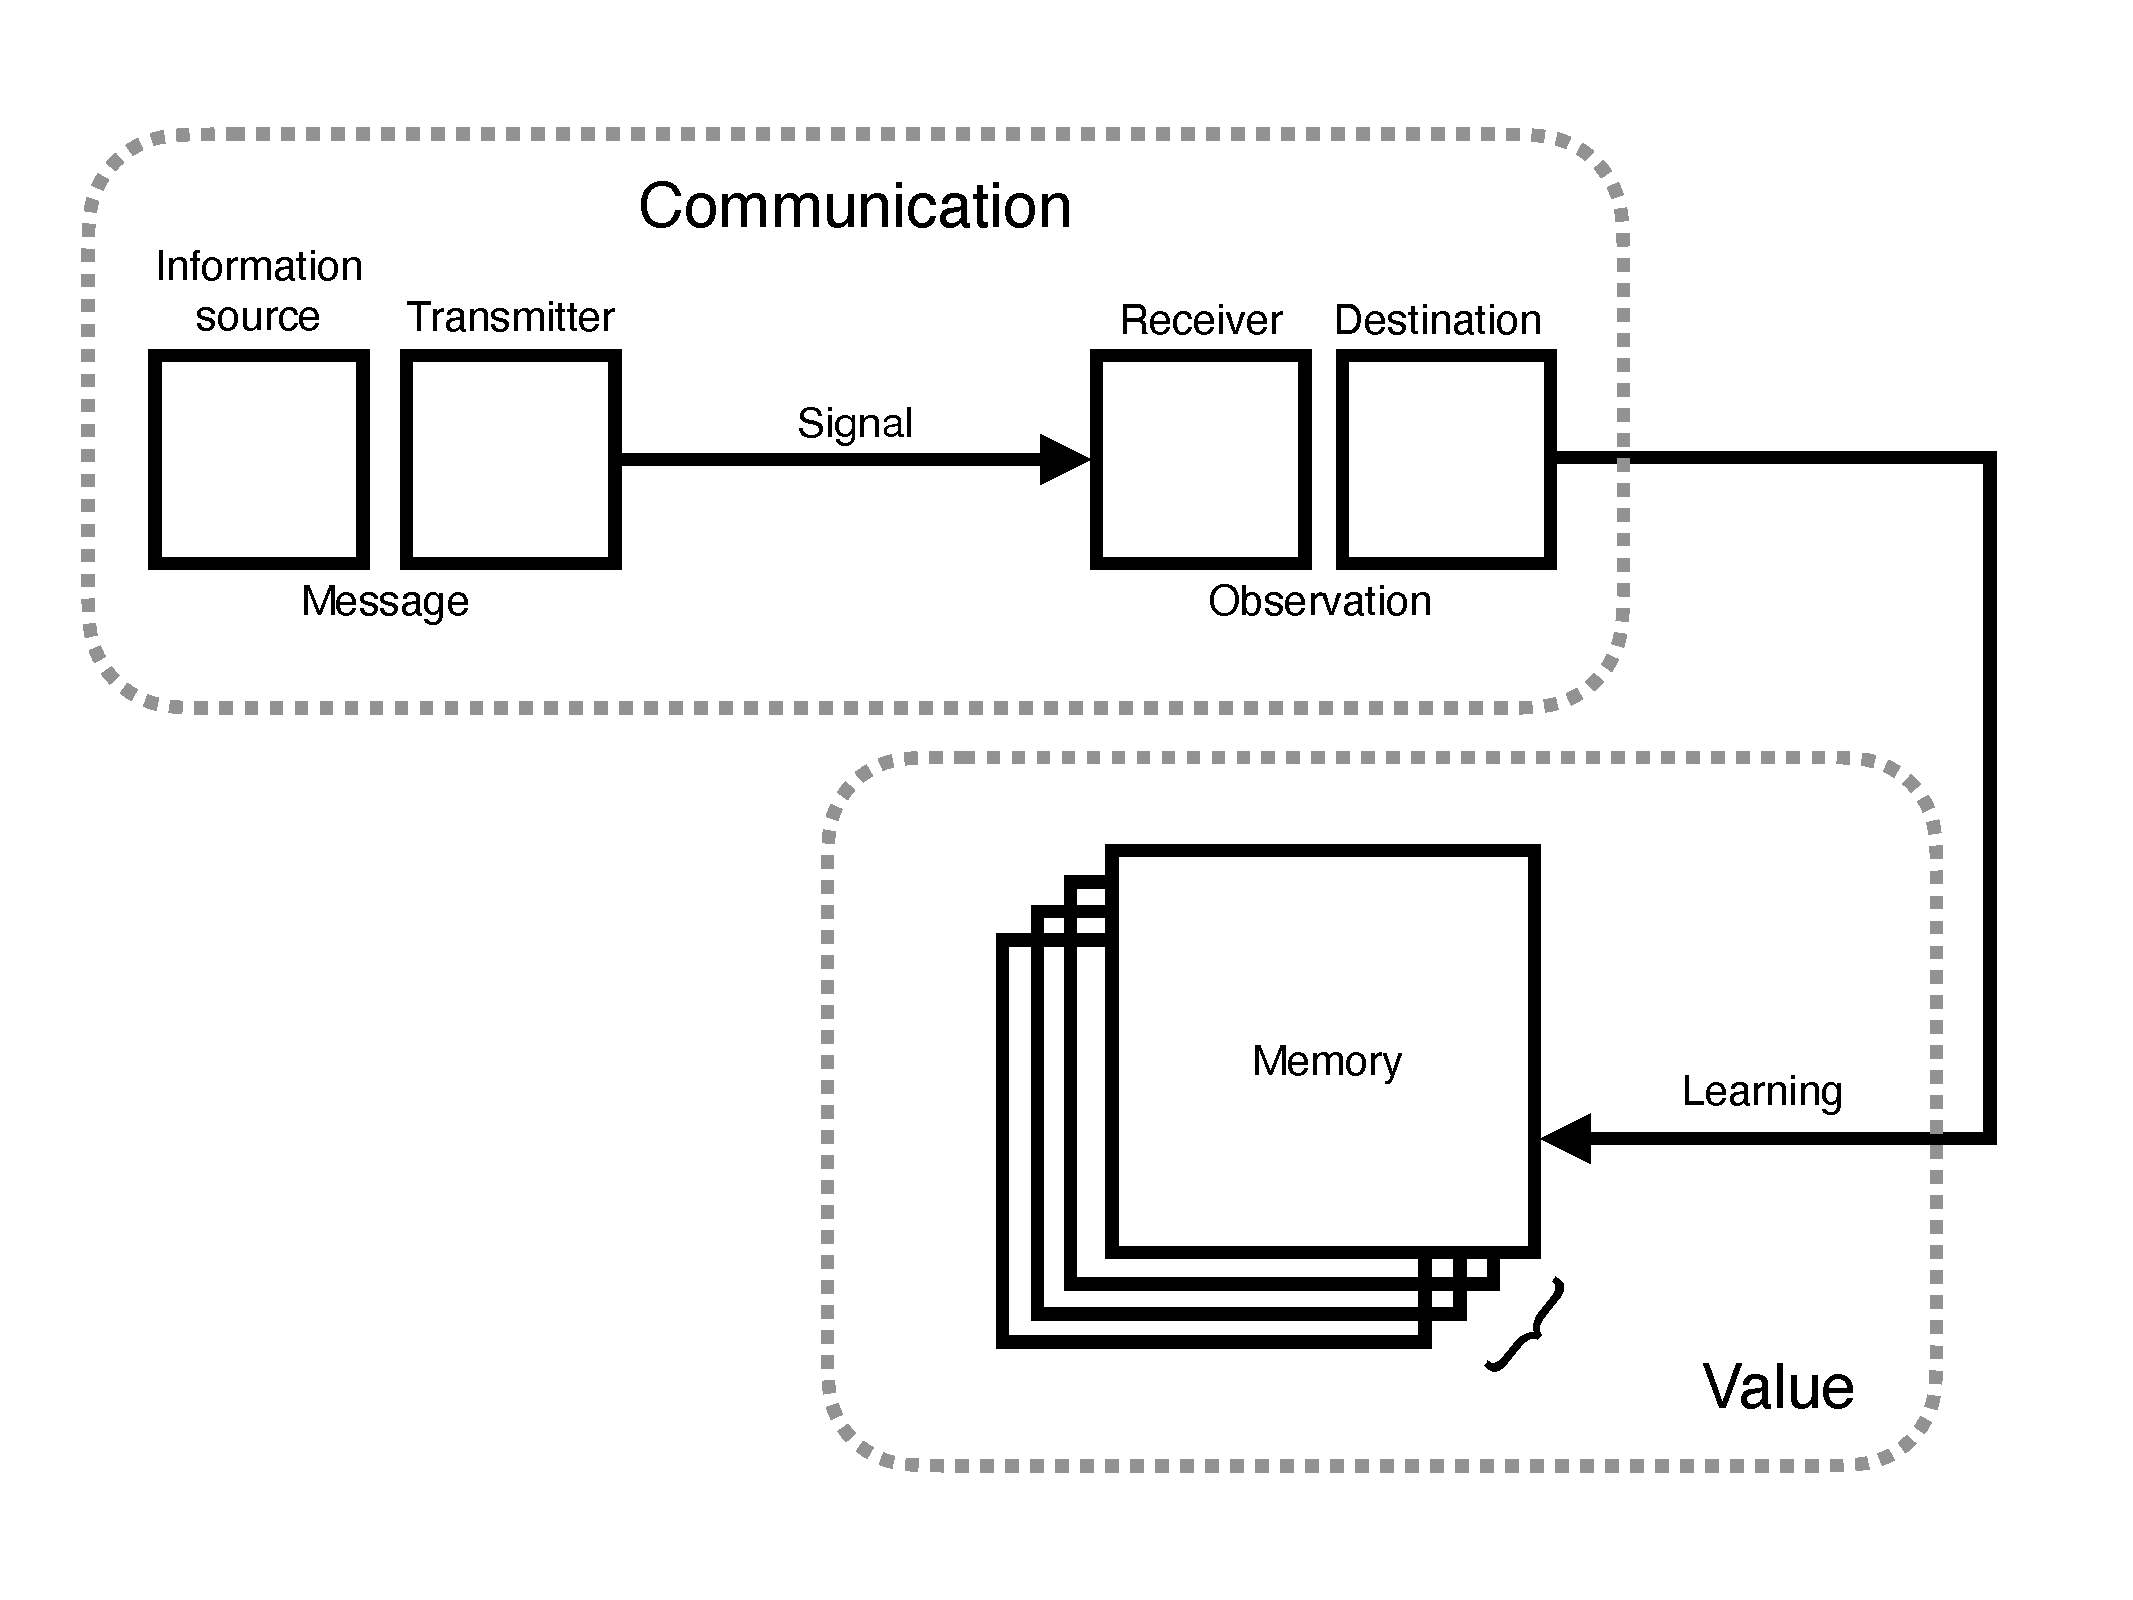
\includegraphics[width=1.0\linewidth]{img/info_diagram.pdf} 
    \caption{The relationship between the technical problem of communication with the technical problem of value. Note how value is not derived from the channel directly. Value is derived from learning about observations from the channel, which is in turn dependent on memory and its past history.
    }
    \label{fig:info1} 
\end{figure}

There is, we argue, an analogous set of levels for information value as those Weaver describes. a. There is the technical problem of judging how much was learned. b. There is the semantic problem of both what this learning ``means'', and also what its consequences are. c. There is an effectiveness problem of using what was learned to some other effect. 

\subsection*{Is this too complex?}
Perhaps turning a single objective into two, as we have, is too complex an answer. If this is true, then it would mean our strategy is not a parsimonious solution to the dilemma. We could or should reject it on that alone?

Questions about parsimony can be sometimes resolved by considering the benefits versus the costs to adding complexity. The benefits to curiosity-based search is that it leads to no regret solutions to exploration, to exploration-exploitation, and that it so far seems to do very well in practice, at reward collection. At the same time curiosity-as-exploration can also be building a model of the environment, useful for later planning \cite{Ahilan2019,Poucet1993}, creativity, imagination \cite{Schmidhuber2010}, while also building, in some cases, diverse action strategies \cite{Lehman2011a,Lehman2013,Mouret2015,Colas2020}. 

The cost is of curiosities indirectness, which could make it slower to converge in principle. There is also the risk of focusing on minutia, which we discuss in the main text. Our numerical simulation suggests neither of these costs are not fatal for finding practical successes.


\subsection*{Is this too simple?}
Solutions to the regular dilemma are complex and require sophisticated mathematical efforts and complex computations, when compared to our solution. Put another way, our solution may seem too simple to some. So have we ``cheated'' by changing the problem in the way that we have?

The truth is we might have cheated, in this sense: the dilemma might have to be as hard as it has seemed. But the general case for curiosity as useful in exploration is clear, and backed up by the brute fact of its widespread presence. The question is: is curiosity so useful and so robust that it can be sufficient for all exploration with learning. 

The answer to this question is empirical. If our account does well in describing and predicting animal behavior, that would be some evidence for it \cite{Sumner2019,Wang2019,Jaegle2019,Gottlieb2018,Kidd2015,Berlyne1950,Colas2020a,Rahnev2018,Wilson2020,CogliatiDezza2017b,Berger-Tal2014}. If it predicts neural structures \cite{Cisek2019,Kobayashi2019}, that would be some evidence for it (we discuss this more below). If this theory proves useful in machine learning and artificial intelligence research, that would be some evidence for it \cite{Burda2018,Schmidhuber1991,deAbril2018,Fister2019,Lehman2011a,Stanley2004a,Colas2020,Cully2015,Wilson2020,Pathak2019}. 


\subsection*{Is this a slight of hand, theoretically?}
Yes. It is often useful in mathematical studies to take one problem that cannot be solved, and replace it with another related problem that can be. In this case, we swap one highly motivated animal behavior (reward seeking) for another (information seeking).


\subsection*{Does value as a technical problem even make sense?}
Having a technical definition of value, free from any meaning, might seem counterintuitive property for a value measure. We argue that it is not more or less counterintuitive than stripping information of meaning in the first  place. The central question for our account of value is, will it prove useful? 


\subsection*{What about mutual information, or truth?}
In other prototypical examples, information value is based on how well what is learned relates to the environment \cite{Behrens2007,Kolchinsky2018,Tishby2000}, that is the mutual information the internal memory and the external environment. Colloquially, one might call this ``truth seeking". 

As a people we pursue information which is fictional \cite{sternisko2020dark}, or based on analogy \cite{gentner1997reasoning}, or outright wrong \cite{loftus1989misinformation}. Conspiracy theories, disinformation, and our many more mundane errors, are far too commonplace for information value to be based on mutual information, as defined above. This does not mean that holding false beliefs cannot harm survival, but this is a second order question as far as learning goes. 


\subsection*{So you suppose there is always positive value for learning of all fictions, disinformation, and deceptions?}
We must. This is our most unexpected prediction. Yet, logically, it is internally consistent with our work we believe qualitatively consistent with the behavior of humans and animals alike. The fact that humans consistently seek to learn false things calls out us to accept that learning alone is a motivation for behavior.


\subsection*{What about information foraging?}
Our work is heavily inspired by information foraging \cite{Inglis2001,Reddy2016}. Our motivation in developing our novel strategy was that information value should not depend on only a probabilistic reasoning, as it does in information foraging. This is for the simple reason that many of the problems animals need to learn are not probabilistic problems \textit{from their point of view}. 


\subsection*{Was it necessary to build a general theory for information value just to describe curiosity?}
No. It was an idealistic choice that worked out. The field of curiosity studies has shown that there are many kinds of curiosity. At the extreme limit of this diversity is a notion of curiosity defined for any kind of observation, and any kind of learning. If we were able to develop a theory of value driven search at this limit, we can be sure it will apply in all possible examples of curiosity that we seem sure to discover in future. At this limit we can also be sure that the ideas will span fields, addressing the problem as it appears in computer science, machine learning, game theory, psychology, neuroscience, biology, and economics.


\subsection*{Doesn't your definition of regret ignore lost rewards when the curiosity policy is in control?}
Yes. Regret is calculated for the policy which is in control of behavior, not the policy which \textit{could} have been in control of behavior.


\subsection*{Is information a reward?}
If reward is defined as more-or-less any quantity that motivates behavior, then our definition of information value is a reward. This last point does not mean, however, that information value and environmental rewards are interchangeable. Rewards from the environment are a conserved resource, information is not. For example, if a rat shares a potato chip with a cage-mate, it must break the chip up leaving it less food for itself. While if a student shares an idea with a classmate, that idea is not divided up. 

Furthermore, if you add reward value and information value to motivate search you can drive exploration in practical and useful ways. But this doesn't change the intractability of the dilemma proper \cite{Thrun1992a,Dayan1996,Findling2018,Gershman2018b}. 

In other words, it depends. 


\subsection*{But isn't curiosity impractical?}
It does seem curiosity is just as likely to lead away from a needed solution as towards it. Especially so if one watches children who are the prototypical curious explorers \cite{Sumner2019,Kidd2015}. This is why we limit curiosity with boredom, and counter it with a competing drive for reward collecting (i.e., exploitation). 

We believe there is a useful analogy between science and engineering. Science can be considered an open-ended inquiry, and engineering a purpose driven enterprise. They each have their own pursuits but they also learn from each other, often in alternating iterations \cite{Gupta2006}. It is their different objectives though which make them such good long-term collaborators.


\subsection*{But what about curiosity on big problems?}
A significant drawback to curiosity, as an algorithm, is that it will struggle to deliver timely results when the problem is very large, or highly detailed. First, it is worth noting that most learning algorithms struggle with this setting \cite{MacKay2003,Sutton2018}, that is unless significant prior knowledge can be brought to bear \cite{Zhang2020,Sutton2018} or the problem can be itself compressed \cite{Ha2018a,Fister2019}. Because ``size'' is a widespread problem in learning, there are a number of possible solutions and because our definition of learning, memory and curiosity is so general, we can take advantage of most. This does not guarantee curiosity will work out for all problems; all learning algorithms have counterexamples \cite{Wolpert1997}. 


\subsection*{But what about other forms of curiosity?}
We did not intend to dismiss the niceties of curiosity that others have revealed. It is that these prior divisions parcel out the idea too soon. Philosophy and psychology consider whether curiosity is internal or external, perceptual versus epistemic, or specific versus diversive, or kinesthetic \cite{Kidd2015,Berlyne1950,Zhou2020}. Computer science tends to define it as needed, for the task at hand \cite{Stanley2004,Lehman2011a,Lehman2013,Mouret2015,Colas2020}. Before creating a taxonomy of curiosity it is important to first define it, mathematically. Something we have done here.


\subsection*{What is boredom, besides being a tunable parameter?}
A more complete version of the theory would let us derive a useful or even optimal value for boredom, if given a learning problem or environment. This would also answer the question of what boredom is computationally. We cannot do this. It is the next problem we will work on, and it is very important. The central challenge is deriving boredom for any kind of learning algorithm.


\subsection*{Does this mean you are hypothesizing that boredom is actively tuned?}
Yes we are predicting exactly that.


\subsection*{But do people subjectively feel they can tune their boredom?}
From our experience, no. Perhaps it happens unconsciously? For example we seem to alter physiological learning rates without subjectively experiencing it \cite{Behrens2007}.


\subsection*{How can an animal tune boredom in a new setting?}
The short answer is that one would need to guess and check. Our work in Fig \ref{fig:robust} suggests that this can be somewhat robust.


\subsection*{Do you have any evidence in animal behavior and neural circuits?}
There is some evidence for our theory of curiosity in psychology and neuroscience, however, in these fields curiosity and reinforcement learning have largely developed as separate disciplines \cite{Berlyne1950,Kidd2015,Sutton2018}. Indeed, we have highlighted how they are separate problems, with links to different basic needs: gathering resources to maintain physiological homeostasis \cite{Keramati2014,Juechems2019} and gathering information to decide what to learn and to plan for the future \cite{Valiant1984,Sutton2018}. Here we suggest that though they are separate problems, they are problems that can, in large part, solve one another. This insight is the central idea to our view of the explore-exploit decisions. 

Yet there are hints of this independent cooperation of curiosity and reinforcement learning out there. Cisek (2019) has traced the evolution of perception, cognition, and action circuits from the Metazoan to the modern age \cite{Cisek2019}. The circuits for reward exploitation and observation-driven exploration appear to have evolved separately, and act competitively, exactly the model we suggest. In particular he notes that exploration circuits in early animals were closely tied to the primary sense organs (i.e. information) and had no input from the homeostatic circuits \cite{Keramati2014,Cisek2019,Juechems2019}. This neural separation for independent circuits has been observed in ``modern'' high animals, including zebrafish \cite{Marques2019} and monkeys \cite{White2019,Wang2019}. 


\subsection*{What about aversive values?}
We certainly do not believe this is a complete theory of rewarding decisions. For example, we do not account for any consequences of learning, or any other aversive events. Accounting for these is another important next step.

The presence of many values fits well within our notion of competition between simple (pure) policies, in a win-stay loose-shift game \cite{Estes1994TowardAS}. To take other values into account we need a different notation, from the inequalities of Eq.~\ref{eq:pipi}. For example, if we added a fear value $F$ to our homeostatic scheme we can move to argmax notation,

\begin{equation}
\label{eq:pipi_f} 
\Pi^{\pi} = \ \Big [ \pi_E,\ \pi_R,\ \pi_F \Big ]
\end{equation}

\begin{equation}
\label{eq:meta_greedy_f} 
	\argmax_{\Pi^{\pi}} \ \Big [ E - \eta,\ \hat R - \rho,\ F + \phi \Big ]
\end{equation}

Adding a bias term to each value provides a direct way to break ties, and set default behaviors. Additional to our standard assumptions, if we also assume the fear/aversive term should take precedence over all other options when there is a tie, then $\phi > \rho > \eta$.

\subsection*{What about other values?}
Another more mundane example would be to add a policy for a grooming drive, $C$. 

\begin{equation}
\label{eq:pipi_c} 
\Pi^{\pi} = \ \Big [ \pi_E,\ \pi_R,\ \pi_C \Big ]
\end{equation}

\begin{equation}
\label{eq:meta_greedy_c} 
\argmax_{\Pi^{\pi}} \ \Big [ E - \eta,\ \hat R - \rho,\ C + \chi \Big ]
\end{equation}

Where we assume the grooming term should take precedence over all other options, when there is a tie. That is, $\chi > \rho > \eta$.

% \subsection*{What about fitting deterministic models?}
% Exploration in the lab is often described as probabilistic \cite{Calhoun2014,Song2019a,Gershman2018b,Schulz2018a}. By definition probabilistic models do not make exact predictions of behavior, only statistical ones. Our approach is deterministic and so can make exact predictions. If, that is, we can fit it and it turns out to be correct. In species ranging from human to \textit{Caenorhabditis elegans}, there are hundreds of exploration-exploitation experiments. A deterministic theory can, in principle, open up entirely new avenues for reanalysis. Testing and exploring these is a critical next step.


\subsection*{Does regret matter?}
Another way around the dilemma is to ignore regret altogether. This is the domain of pure exploration methods, like the Gitten’s Index \cite{Gittins1979}, or probably-approximately correct approaches \cite{Valiant1984}, or other bounded forms of reinforcement learning \cite{Brafman2002}. Such methods can guarantee that you find the best reward value actions, eventually. These methods do not consider regret, as we have. But we argue that regret is critical to consider when resources and time are scarce, as they are in most natural settings. 



\subsection*{Is the algorithmic run time practical?}
It is common in computer science to study the run time of an algorithm as a measure of its efficiency. So what is the run time of our win stay, loose switch solution? There is unfortunately no fixed answer for the average or best case. The worst case algorithmic run time is linear and additive in the independent policies. If it takes $T_E$ steps for $\pi_E$ to converge, and $T_R$ steps for $\pi_R$, then the worst case run time for $\pi_{\pi}$ is $T_E + T_R$. Of course this is the worst case run time and would still be within reasonable ranges for learning in most naturalistic contexts.

\subsection*{What predictions does this theory make?}
In what sense can your mathematical union be tested? Normally, to test a model or theory of learning one tests whether or not the learning algorithm appears to be at work in the animal of interest. However our axioms, and their learning rule independence, means nearly any rule will do. Testing must therefore be qualitative, for which we have four strong predictions to make. 

% TODO - add Diss of Rosenburg and supporting data that exists. Add it in each number.

\begin{enumerate}
    \item \textbf{Invariant exploration strategy}. The presence of reward should not change the exploration strategy. This is tricky, because differing sense information is often associated with the presence of absence of reward. This sense of information would in many cases change learning and so change curious exploration. \emph{Auxiliary assumptions}. Learning is possible because there is some novelty ($\hat E > \eta$), and some observations available to learn from. These criteria rule out for example situations where Levy walks would be optimal \cite{Viswanathan2000}.
    \item \textbf{Information preference following reward absence}. When reward is absent, an animal should immediately choose to do an information collection with it's next action. \emph{Auxiliary assumptions}. Learning is possible because there is some novelty ($\hat E > \eta$), and some observations available to learn from.
    \item \textbf{Deterministic search}. Read strictly, environmental noise is the only source of noise in our models exploration behavior. To evaluate this we must move from population-level distribution analysis, to moment-by-moment predation of animal behavior \cite{Peters2016,Mangalam2021}. \emph{Auxiliary assumptions}. perfect memory, no forgetting, or action/parameter/neural noise.
    \item  \textbf{Well defined pure-periods}. There should be a well defined period of exploration and exploitation. \emph{Auxiliary assumptions}. There are no other behaviors, are driving factors, present. For example, learning fear, avoiding, or grooming.
\end{enumerate}

Of course the presence of any four criteria does not indicate our theory is at work, mechanistically. Mechanistic claims for any biological or behavioral problems are difficult if not impossible to be certain of. Instead, we view meeting each of these criteria as some evidence for our account. We think the nice mathematical properties of our union makes it a good general candidate for solving explore-exploit problems, and ultimately we wish to test how true that is.  

% Kidd U. 
% Relation to count based search
% Noise tuning? See Wilson?
% Noise, and predation.

\subsection*{Summary}
We have argued one can put aside any intuitions that suggest a curious search is too inefficient, or open-ended, to be practical for reward collection. We have shown it can be made very practical, and mathematically optimal. We have shown there is a zero-regret way to solve the dilemma, a problem that has seemed unsolvable in those terms. Simply, be curious.


